\documentclass{ximera}

\usepackage{epsfig}

\graphicspath{
  {./}
  {figures/}
}


\usepackage{morewrites}

%\newcounter{ccounter}
%\setcounter{ccounter}{1}
%\newcommand{\Chapter}[1]{\setcounter{chapter}{\arabic{ccounter}}\chapter{#1}\addtocounter{ccounter}{1}}

%\newcommand{\section}[1]{\section{#1}\setcounter{thm}{0}\setcounter{equation}{0}}

%\renewcommand{\theequation}{\arabic{chapter}.\arabic{section}.\arabic{equation}}
%\renewcommand{\thefigure}{\arabic{chapter}.\arabic{figure}}
%\renewcommand{\thetable}{\arabic{chapter}.\arabic{table}}

%\newcommand{\Sec}[2]{\section{#1}\markright{\arabic{ccounter}.\arabic{section}.#2}\setcounter{equation}{0}\setcounter{thm}{0}\setcounter{figure}{0}}

\newcommand{\Sec}[2]{\section{#1}}

\setcounter{secnumdepth}{2}
%\setcounter{secnumdepth}{1} 

%\newcounter{THM}
%\renewcommand{\theTHM}{\arabic{chapter}.\arabic{section}}

\newcommand{\trademark}{{R\!\!\!\!\!\bigcirc}}
%\newtheorem{exercise}{}

\newcommand{\dfield}{{\sf dfield9}}
\newcommand{\pplane}{{\sf pplane9}}

\newcommand{\EXER}{\section*{Exercises}}%\vspace*{0.2in}\hrule\small\setcounter{exercise}{0}}
\newcommand{\CEXER}{}%\vspace{0.08in}\begin{center}Computer Exercises\end{center}}
\newcommand{\TEXER}{} %\vspace{0.08in}\begin{center}Hand Exercises\end{center}}
\newcommand{\AEXER}{} %\vspace{0.08in}\begin{center}Hand Exercises\end{center}}

% BADBAD: \newcommand{\Bbb}{\bf}

\newcommand{\R}{\mbox{$\Bbb{R}$}}
\newcommand{\C}{\mbox{$\Bbb{C}$}}
\newcommand{\Z}{\mbox{$\Bbb{Z}$}}
\newcommand{\N}{\mbox{$\Bbb{N}$}}
\newcommand{\D}{\mbox{{\bf D}}}
\usepackage{amssymb}
%\newcommand{\qed}{\hfill\mbox{\raggedright$\square$} \vspace{1ex}}
%\newcommand{\proof}{\noindent {\bf Proof:} \hspace{0.1in}}

\newcommand{\setmin}{\;\mbox{--}\;}
\newcommand{\Matlab}{{M\small{AT\-LAB}} }
\newcommand{\Matlabp}{{M\small{AT\-LAB}}}
\newcommand{\computer}{\Matlab Instructions}
\newcommand{\half}{\mbox{$\frac{1}{2}$}}
\newcommand{\compose}{\raisebox{.15ex}{\mbox{{\scriptsize$\circ$}}}}
\newcommand{\AND}{\quad\mbox{and}\quad}
\newcommand{\vect}[2]{\left(\begin{array}{c} #1_1 \\ \vdots \\
 #1_{#2}\end{array}\right)}
\newcommand{\mattwo}[4]{\left(\begin{array}{rr} #1 & #2\\ #3
&#4\end{array}\right)}
\newcommand{\mattwoc}[4]{\left(\begin{array}{cc} #1 & #2\\ #3
&#4\end{array}\right)}
\newcommand{\vectwo}[2]{\left(\begin{array}{r} #1 \\ #2\end{array}\right)}
\newcommand{\vectwoc}[2]{\left(\begin{array}{c} #1 \\ #2\end{array}\right)}



\newcommand{\inv}{^{-1}}
\newcommand{\CC}{{\cal C}}
\newcommand{\CCone}{\CC^1}
\newcommand{\Span}{{\rm span}}
\newcommand{\rank}{{\rm rank}}
\newcommand{\trace}{{\rm tr}}
\newcommand{\RE}{{\rm Re}}
\newcommand{\IM}{{\rm Im}}
\newcommand{\nulls}{{\rm null\;space}}

\newcommand{\dps}{\displaystyle}
\newcommand{\arraystart}{\renewcommand{\arraystretch}{1.8}}
\newcommand{\arrayfinish}{\renewcommand{\arraystretch}{1.2}}
\newcommand{\Start}[1]{\vspace{0.08in}\noindent {\bf Section~\ref{#1}}}
\newcommand{\exer}[1]{\noindent {\bf \ref{#1}}}
\newcommand{\ans}{}
\newcommand{\matthree}[9]{\left(\begin{array}{rrr} #1 & #2 & #3 \\ #4 & #5 & #6
\\ #7 & #8 & #9\end{array}\right)}
\newcommand{\cvectwo}[2]{\left(\begin{array}{c} #1 \\ #2\end{array}\right)}
\newcommand{\cmatthree}[9]{\left(\begin{array}{ccc} #1 & #2 & #3 \\ #4 & #5 &
#6 \\ #7 & #8 & #9\end{array}\right)}
\newcommand{\vecthree}[3]{\left(\begin{array}{r} #1 \\ #2 \\
#3\end{array}\right)}
\newcommand{\cvecthree}[3]{\left(\begin{array}{c} #1 \\ #2 \\
#3\end{array}\right)}
\newcommand{\cmattwo}[4]{\left(\begin{array}{cc} #1 & #2\\ #3
&#4\end{array}\right)}

\newcommand{\Matrix}[1]{\ensuremath{\left(\begin{array}{rrrrrrrrrrrrrrrrrr} #1 \end{array}\right)}}

\newcommand{\Matrixc}[1]{\ensuremath{\left(\begin{array}{cccccccccccc} #1 \end{array}\right)}}



\renewcommand{\labelenumi}{\theenumi)}
\newenvironment{enumeratea}%
{\begingroup
 \renewcommand{\theenumi}{\alph{enumi}}
 \renewcommand{\labelenumi}{(\theenumi)}
 \begin{enumerate}}
 {\end{enumerate}\endgroup}



\newcounter{help}
\renewcommand{\thehelp}{\thesection.\arabic{equation}}

%\newenvironment{equation*}%
%{\renewcommand\endequation{\eqno (\theequation)* $$}%
%   \begin{equation}}%
%   {\end{equation}\renewcommand\endequation{\eqno \@eqnnum
%$$\global\@ignoretrue}}

%\input{psfig.tex}

\author{Martin Golubitsky and Michael Dellnitz}

%\newenvironment{matlabEquation}%
%{\renewcommand\endequation{\eqno (\theequation*) $$}%
%   \begin{equation}}%
%   {\end{equation}\renewcommand\endequation{\eqno \@eqnnum
% $$\global\@ignoretrue}}

\newcommand{\soln}{\textbf{Solution:} }
\newcommand{\exercap}[1]{\centerline{Figure~\ref{#1}}}
\newcommand{\exercaptwo}[1]{\centerline{Figure~\ref{#1}a\hspace{2.1in}
Figure~\ref{#1}b}}
\newcommand{\exercapthree}[1]{\centerline{Figure~\ref{#1}a\hspace{1.2in}
Figure~\ref{#1}b\hspace{1.2in}Figure~\ref{#1}c}}
\newcommand{\para}{\hspace{0.4in}}

\renewenvironment{solution}{\suppress}{\endsuppress}

\ifxake
\newenvironment{matlabEquation}{\begin{equation}}{\end{equation}}
\else
\newenvironment{matlabEquation}%
{\let\oldtheequation\theequation\renewcommand{\theequation}{\oldtheequation*}\begin{equation}}%
  {\end{equation}\let\theequation\oldtheequation}
\fi

\makeatother


\title{m15.tex}

\begin{document}
\begin{abstract}
BADBAD
\end{abstract}
\maketitle

\chapter{Linear Differential Equations}


\subsection*{Section~\protect{\ref{S:SEOC}} Solving Systems in Original Coordinates}
\rhead{S:SEOC}{SOLVING SYSTEMS IN ORIGINAL COORDINATES}


\exer{c12.1.2a} \ans
\[
X_1(t) = e^{2t}\vectwo{1}{0} \AND
X_2(t) = e^{2t}\vectwo{t}{1}
\]
are linearly independent solutions to $\dot{X} = AX$.

\soln First find the eigenvalues of $A$.  Since $A$ is upper triangular,
the eigenvalues are the diagonal entries.  Therefore $\lambda_1 = 2$
is a double eigenvalue.  Then solve $(A - \lambda_1 I_2)w_1 = 0$ to
find that $w_1 = (1,0)^t$ is an eigenvector of $A$.  Find a
generalized eigenvector $w_2$ such that $(A - \lambda_1 I_2)w_2 =
w_1$, in this case, $w_2 = (0,1)^t$.  Now, by \Ref{E:Xj},
there are linearly independent solutions $X_1(t)$ and $X_2(t)$ such that
\[
\begin{array}{rcl}
X_1(t) & = & e^{\lambda_1 t}w_1 = e^{2t}\vectwo{1}{0} \\ X_2(t) & = &
e^{\lambda_1 t}(tw_1 + w_2) = e^{2t}\left(\vectwo{t}{0} +
\vectwo{0}{1}\right).
\end{array}
\]

\exer{c12.1.2b} \ans
\[
X_1(t) = \cvecthree{e^t}{0}{0}, \quad
X_2(t) = \cvecthree{0}{e^{-t}}{0}, \AND
X_3(t) = e^{-t}\cvecthree{0}{t + 1}{\frac{1}{2}}
\]
are linearly independent solutions to $\dot{X} = AX$.

\soln The eigenvalues of $A$ are the diagonal entries, since $A$ is upper
triangular.  For each eigenvalue, solve $(A - \lambda_j I_2)w_j = 0$
to find that $\lambda_1 = 1$ is an eigenvalue with eigenvector $w_1 =
(1,0,0)^t$, and that $\lambda_2 = -1$ is a double eigenvalue with
single eigenvector $w_2 = (0,1,0)^t$.  Find $w_3$, the generalized
eigenvector for $\lambda_2$, by solving $(A - \lambda_2 I_3)w_3 = w_2$
to obtain $w_3 = (0,1,\frac{1}{2})^t$.  Now, by \Ref{E:Xj},
there are linearly independent solutions $X_j(t)$ such that
\[
\begin{array}{rcl}
X_1(t) & = & e^{\lambda_1 t}w_1 = e^t\vecthree{1}{0}{0} \\
X_2(t) & = & e^{\lambda_2 t}w_2 = e^{-t}\vecthree{0}{1}{0} \\
X_3(t) & = & e^{\lambda_2 t}(tw_2 + w_3) = e^{-t}\left(\vecthree{0}{t}{0}
+ \vecthree{0}{1}{\frac{1}{2}}\right).
\end{array}
\]

\exer{c12.1.2c} \ans
\[
X_1(t) = e^{2t}\vectwo{1}{-1} \AND
X_2(t) = e^{2t}\cvectwo{t - 1}{-t}
\]
are linearly independent solutions to $\dot{X} = AX$.

\soln First find the eigenvalues of $A$.  In this case, $\lambda_1 = 2$
is a double eigenvalue.  Then solve $(A - \lambda_1 I_2)w_1 = 0$ to
find that $w_1 = (1,-1)^t$ is an eigenvector of $A$.  Find a
generalized eigenvector $w_2$ such that $(A - \lambda_1 I_2)w_2 =
w_1$, in this case, $w_2 = (-1,0)^t$.  Now, by \Ref{E:Xj},
there are linearly independent solutions $X_1(t)$ and $X_2(t)$ such that
\[
\begin{array}{rcl}
X_1(t) & = & e^{\lambda_1 t}w_1 = e^{2t}\vectwo{1}{-1} \\
X_2(t) & = & e^{\lambda_1 t}(tw_1 + w_2) = e^{2t}\left(\vectwo{t}{-t} +
\vectwo{-1}{0}\right).
\end{array}
\]

\exer{c12.1.2d} \ans
\[
X_1(t) = e^{-4t}\vecthree{1}{0}{1}, \quad
X_2(t) = e^{5t}\vecthree{0}{0}{1}, \AND
X_3(t) = e^{5t}\vecthree{-1}{1}{t}
\]
are linearly independent solutions to $\dot{X} = AX$.

\soln First find the eigenvalues and eigenvectors of $A$.  In this case,
$A$ has an eigenvalue at $\lambda_1 = -4$ with eigenvector $w_1 =
(1,0,1)^t$, and a double eigenvalue at $\lambda_2 = 5$ with single
eigenvector $w_2 = (0,0,1)^t$.  Find $w_3$, the generalized
eigenvector for $\lambda_2$, by solving $(A - \lambda_2 I_3)w_3 = w_2$
to obtain $w_3 = (-1,1,0)^t$.  Now, by \Ref{E:Xj},
there are linearly independent solutions $X_j(t)$ such that
\[
\begin{array}{rcl}
X_1(t) & = & e^{\lambda_1 t}w_1 = e^{-4t}\vecthree{1}{0}{1} \\
X_2(t) & = & e^{\lambda_2 t}w_2 = e^{5t}\vecthree{0}{0}{1} \\
X_3(t) & = & e^{\lambda_2 t}(tw_2 + w_3) = e^{5t}\left(\vecthree{0}{0}{t}
+ \vecthree{-1}{1}{0}\right).
\end{array}
\]

\exer{c12.1.6a} \ans
\[
e^{tA} = -e^t\frac{1}{2}\mattwo{1}{1}{1}{1} +
e^{-t}\frac{1}{2}\mattwo{-1}{1}{1}{-1}
= -\frac{1}{2}\cmattwo{e^{t} + e^{-t}}{e^t - e^{-t}}{e^t - e^{-t}}
{e^t + e^{-t}}.
\]

\soln First find the eigenvalues of $A$, which are $\lambda_1 = 1$ and
$\lambda_2 = -1$.  By Corollary~\ref{T:etA0},
\[
e^{tA} = \sum_{\ell = 1}^2 e^{\lambda_\ell t}a_\ell(A)P_\ell(A).
\]
The characteristic polynomial of $A$ is $p_A(\lambda) = (\lambda -
1)(\lambda + 1)$, so $P_1(\lambda) = \lambda + 1$ and $P_2(\lambda) =
\lambda - 1$.  Use partial fractions to find that
\[
\frac{1}{p_A(\lambda)} = \frac{-\frac{1}{2}}{1 - \lambda} + \frac{\frac{1}{2}}
{-1 - \lambda}.
\]
Thus, $a_1(\lambda) = -\frac{1}{2}$ and $a_2(\lambda) = \frac{1}{2}$.  So
\[
\begin{array}{rcl}
e^{tA} & = & e^ta_1(A)P_1(A) + e^{-t}a_2(A)P_2(A) \\
& = & \dps e^t\left(-\frac{1}{2}\right)\left(\mattwo{0}{1}{1}{0} +
\mattwo{1}{0}{0}{1}\right) + e^{-t}\left(\frac{1}{2}\right)
\left(\mattwo{0}{1}{1}{0} - \mattwo{1}{0}{0}{1}\right).
\end{array}
\]

\exer{c12.1.6b} \ans
\[
e^{tA} = -e^{3t}\frac{1}{2}\mattwo{1}{1}{1}{1} +
e^t\frac{1}{2}\mattwo{-1}{1}{1}{-1}
= -\frac{1}{2}\cmattwo{e^{3t} + e^{t}}{e^{3t} - e^{t}}{e^{3t} - e^{t}}
{e^{3t} + e^{t}}.
\]

\soln First find the eigenvalues of $A$, which are $\lambda_1 = 3$ and
$\lambda_2 = 1$.  By Corollary~\ref{T:etA0},
\[
e^{tA} = \sum_{\ell = 1}^2 e^{\lambda_\ell t}a_\ell(A)P_\ell(A).
\]
The characteristic polynomial of $A$ is $p_A(\lambda) = (\lambda -
1)(\lambda - 3)$, so $P_1(\lambda) = \lambda - 1$ and $P_2(\lambda) =
\lambda - 3$.  Use partial fractions to find that
\[
\frac{1}{p_A(\lambda)} = \frac{-\frac{1}{2}}{3 - \lambda} + \frac{\frac{1}{2}}
{1 - \lambda}.
\]
Thus, $a_1(\lambda) = -\frac{1}{2}$ and $a_2(\lambda) = \frac{1}{2}$.  So
\[
\begin{array}{rcl}
e^{tA} & = & e^ta_1(A)P_1(A) + e^{-t}a_2(A)P_2(A) \\
& = & \dps e^{3t}\left(-\frac{1}{2}\right)\left(\mattwo{2}{1}{1}{2} -
\mattwo{1}{0}{0}{1}\right) + e^{t}\left(\frac{1}{2}\right)
\left(\mattwo{2}{1}{1}{2} - \mattwo{3}{0}{0}{3}\right).
\end{array}
\]

\exer{c12.1.6c} \ans
\[
e^{tA} = -e^{3t}\frac{1}{2}\mattwo{2}{2}{0}{0} +
e^t\frac{1}{2}\mattwo{0}{2}{0}{-2}
= -\cmattwo{e^{3t}}{e^{3t} - e^{t}}{0}{e^{t}}.
\]

\soln First find the eigenvalues of $A$, which are $\lambda_1 = 3$ and
$\lambda_2 = 1$.  By Corollary~\ref{T:etA0},
\[
e^{tA} = \sum_{\ell = 1}^2 e^{\lambda_\ell t}a_\ell(A)P_\ell(A).
\]
The characteristic polynomial of $A$ is $p_A(\lambda) = (\lambda -
1)(\lambda - 3)$, so $P_1(\lambda) = \lambda - 1$ and $P_2(\lambda) =
\lambda - 3$.  Use partial fractions to find that
\[
\frac{1}{p_A(\lambda)} = \frac{-\frac{1}{2}}{3 - \lambda} + \frac{\frac{1}{2}}
{1 - \lambda}.
\]
Thus, $a_1(\lambda) = -\frac{1}{2}$ and $a_2(\lambda) = \frac{1}{2}$.  So
\[
\begin{array}{rcl}
e^{tA} & = & e^ta_1(A)P_1(A) + e^{-t}a_2(A)P_2(A) \\
& = & \dps e^{3t}\left(-\frac{1}{2}\right)\left(\mattwo{3}{2}{0}{1} -
\mattwo{1}{0}{0}{1}\right) + e^{t}\left(\frac{1}{2}\right)
\left(\mattwo{3}{2}{0}{1} - \mattwo{3}{0}{0}{3}\right).
\end{array}
\]


\exer{c12.1.6d} \ans
\[
e^{tA} =
\cmatthree{e^t}{-e^t + e^{-2t}}{2e^{3t} - e^t + e^{-2t}}
{0}{e^{-2t}}{-e^{3t} + e^{-2t}}
{0}{0}{e^{3t}}.
\]

\soln The characteristic polynomial of $A$ is
$p_A(\lambda) = (\lambda - 3)(\lambda - 1)(\lambda + 2)$, so the
eigenvalues are $\lambda_1 = 3$, $\lambda_2 = 1$, and $\lambda_3 = -2$.
By Corollary~\ref{T:etA0},
\[
e^{tA} = \sum_{\ell = 3}^2 e^{\lambda_\ell t}a_\ell(A)P_\ell(A).
\]
From the characteristic polynomial $p_A(\lambda)$, compute
\[
P_1(\lambda) = \lambda^2 + \lambda - 2, \quad
P_2(\lambda) = \lambda^2 - \lambda - 6, \AND
P_3(\lambda) = \lambda^2 - 4\lambda + 3.
\]
Use partial fractions to find that
\[
\frac{1}{p_A(\lambda)} =
\frac{\frac{1}{5}\lambda - \frac{1}{2}}{P_1(\lambda)}
+ \frac{-\frac{1}{6}\lambda}{P_2(\lambda)}
+ \frac{-\frac{1}{30}\lambda}{P_3(\lambda)}.
\]
Thus
\[
a_1(\lambda) = \frac{1}{5}\lambda - \frac{1}{2}, \quad
a_2(\lambda) = -\frac{1}{6}\lambda, \AND
a_3(\lambda) = -\frac{1}{30}\lambda.
\]
So,
\[
\begin{array}{rcl}
e^{tA} & = & e^{\lambda_1 t}a_1(A)P_1(A) + e^{\lambda_2 t}a_2(A)P_2(A)
+ e^{\lambda_3 t}a_3(A)P_3(A) \\
& = &
\begin{array}{l} e^{3t}(\frac{1}{5}A - \frac{1}{2})(A^2 + A - 2I_3)
+ e^t(-\frac{1}{6}A)(A^2 - A - 6I_3) \\
+\; e^{-2t}(-\frac{1}{30}A)(A^2 - 4A + 3I_2) \end{array} \\
& = & e^{3t}\matthree{0}{0}{2}{0}{0}{-1}{0}{0}{1}
+ e^t\matthree{1}{-1}{-3}{0}{0}{0}{0}{0}{0}
+ e^{-2t}\matthree{0}{1}{1}{0}{1}{1}{0}{0}{0}.
\end{array}
\]

\exer{c12.1.10a} \ans The solution to the given initial value problem is
\[
X(t) = -e^{-t}\vecthree{4}{-1}{6} +
3\vecthree{1}{0}{1} + e^t\vecthree{2}{1}{2}
= \cvecthree{-4e^{-t} + 3 + 2e^t}{e^{-t} + e^t}{-6e^{-t} + 3 + 2e^t}.
\]

\soln The eigenvalues of $A$ are $\lambda_1 = -1$, $\lambda_2 = 0$, and
$\lambda_3 = 1$, with associated eigenvectors $w_1 = (4,-1,6)^t$,
$w_2 = (1,0,1)^t$, and $w_3 = (2,1,2)^t$.  So,
\[
\begin{array}{c}
X_1(t) = e^{\lambda_1 t}w_1 = e^{-t}\vecthree{4}{-1}{6}, \quad
X_2(t) = e^{\lambda_2 t}w_2 = \vecthree{1}{0}{1}, \\
X_3(t) = e^{\lambda_3 t}w_3 = e^t\vecthree{2}{1}{2}
\end{array}
\]
are linearly independent solutions.  The general solution is a linear
combination of the $X_j(t)$, and the solution to the initial value
problem $X_0 = X(0)$ satisfies
\[
\vecthree{1}{2}{-1} = X(0) = \alpha_1w_1 + \alpha_2w_2 + \alpha_3w_3
= \alpha_1\vecthree{4}{-1}{6} + \alpha_2\vecthree{1}{0}{1}
+ \alpha_3\vecthree{2}{1}{2}.
\]
Solve this linear system to obtain $\alpha_1 = -1$,
$\alpha_2 = 3$, and $\alpha_3 = 1$.


\exer{c12.1.10b} \ans The solution to the given initial value problem is
\[
X(t) = e^t\vecthree{1}{0}{2} + e^{-t}\vecthree{0}{1}{0} -
e^{-t}\vecthree{1}{t}{1} =
\cvecthree{e^t - e^{-t}}{(1 - t)e^{-t}}{2e^t - e^{-t}}.
\]

\soln The matrix $A$ has an eigenvalue at $\lambda_1 = 1$ with associated
eigenvector $w_1 = (1,0,2)^t$ and a double eigenvalue at $\lambda_2 = -1$
with eigenvector $w_2 = (0,1,0)^t$.  Find a generalized eigenvector at
$\lambda_2$ by solving the equation $(A - \lambda_2I_3)w_3 = w_2$, obtaining
$w_3 = (1,0,1)^t$.  Thus,
\[
\begin{array}{c}
X_1(t) = e^{\lambda_1 t}w_1 = e^{t}\vecthree{1}{0}{2}, \quad
X_2(t) = e^{\lambda_2 t}w_2 = e^{-t}\vecthree{0}{1}{0}, \\
X_3(t) = e^{\lambda_2 t}(w_2t + w_3) = e^{-t}\vecthree{1}{t}{1}
\end{array}
\]
are linearly independent solutions.  The general solution is a linear
combination of the $X_j(t)$, and the solution to the initial value
problem $X_0 = X(0)$ satisfies
\[
\vecthree{0}{1}{1} = X(0) = \alpha_1w_1 + \alpha_2w_2 + \alpha_3w_3
= \alpha_1\vecthree{1}{0}{2} + \alpha_2\vecthree{0}{1}{0}
+ \alpha_3\vecthree{1}{0}{1}.
\]
Solve this linear system to obtain $\alpha_1 = 1$,
$\alpha_2 = 1$, and $\alpha_3 = -1$.

\exer{c12.1.8a} \ans $e^{tA} = \mattwo{1}{t}{0}{1}$.

\soln The matrix $A = \mattwo{0}{1}{0}{0}$ has an eigenvalue $0$ with
multiplicity two.  Theorem~\ref{T:etA} states that 
\[
e^{tA} = a_1(A)P_1(A)\sum_{j=0}^1t^jA^j= a_1(A)P_1(A)(I_2+tA).
\]
In this case $P_1(\lambda)=1=a_1(\lambda)$.   Therefore,
\[
e^{tA} = I_2+tA = \mattwo{1}{t}{0}{1}.
\]


\exer{c12.1.8b} \ans $e^{tA} = e^{-t}\mattwo{1}{2t}{0}{1}$.

\soln The matrix $A = \mattwo{-1}{2}{0}{-1}$ has an eigenvalue $-1$ with
multiplicity two.  Theorem~\ref{T:etA} states that 
\[
e^{tA} = a_1(A)P_1(A)\sum_{j=0}^1e^{-t}t^j(A+I_2)^j=
a_1(A)P_1(A)e^{-t}(I_2+t(A+I_2)).
\]
In this case $P_1(\lambda)=1=a_1(\lambda)$.   Therefore,
\[
e^{tA} = e^{-t}(I_2+t(A+I_2)) = e^{-t}\mattwo{1}{2t}{0}{1}.
\]


\exer{c12.1.8c} \ans $e^{tA}= \dps\frac{1}{4}\left(\begin{array}{rrc} 
1 & -1 & -2+2t\\ -1 & 1 & -2t \\ 0 & 0 & 2\end{array}\right) +e^{2t}\left(\begin{array}{rrr} 2 & 2 & 2\\  2 & 2 & 2 \\ 0 & 0 & 0 
\end{array}\right)$.

\soln The matrix 
$A = \left(\begin{array}{rrr} 1 & 1 & 2\\ 1 & 1 & 0 \\ 0 & 0 & 0
\end{array}\right)$ has eigenvalues $0$ with multiplicity two and $2$ 
with multiplicity one. Theorem~\ref{T:etA} states that 
\begin{eqnarray*}
e^{tA} & = & a_1(A)P_1(A)\sum_{j=0}^1t^jA^j + e^{2t}a_2(A)P_2(A)\\
 & = & a_1(A)P_1(A)(I_3+tA) + e^{2t}a_2(A)P_2(A).
\end{eqnarray*}
The characteristic polynomial of $A$ is $p_A(\lambda) =(2-\lambda)\lambda^2$.
From \Ref{e:Pj} we see that
\[
P_1(\lambda) = 2-\lambda \AND P_2(\lambda) = \lambda^2.
\]
We recall from \Ref{e:1/p} that 
\[
\frac{1}{p_A(\lambda)} = \frac{a_1(\lambda)}{2-\lambda} + 
\frac{a_2(\lambda)}{\lambda^2} = \frac{\frac{1}{4}}{2-\lambda}
+ \frac{\frac{1}{2}+\frac{1}{4}\lambda}{\lambda^2}.
\]
Therefore
\[
a_1(\lambda) = \frac{1}{4} \AND a_2(\lambda) = \frac{1}{2}+\frac{1}{4}\lambda,
\]
and
\begin{eqnarray*}
e^{tA} & = & \frac{1}{4}(2I_3-A)(I_3+tA) + 
e^{2t}\left(\frac{1}{2}I_3+\frac{1}{4}A\right)A^2\\
& = & \frac{1}{4}\left((2I_3-A)+t(2A-A^2)+e^{2t}(2A^2+A^3)\right).
\end{eqnarray*}
Hence
\[
e^{tA}= \frac{1}{4}\left(\left(\begin{array}{rrr} 1 & -1 & -2\\ -1 & 1 & 0 
\\ 0 & 0 & 2\end{array}\right)+t\left(\begin{array}{rrr} 0 & 0 & 2\\ 0 & 0 & -2
\\ 0 & 0 & 0 \end{array}\right)+e^{2t}\left(\begin{array}{rrr} 8 & 8 & 8\\ 
8 & 8 & 8 \\ 0 & 0 & 0\end{array}\right)\right).
\]

\newpage
\exer{c12.1.8d} \ans $e^{tA}= \dps\frac{1}{9}e^{2t}\left(\begin{array}{rcr} 
0 & -2-6t & 6\\ 0 & -3 & 0\\ 0 & 1+3t & -3\end{array}\right) 
+e^{-t}\left(\begin{array}{rrr} -6 & 0 & -12\\  0 & 0 & 0 \\ 0 & 0 & 0 
\end{array}\right)$.


\soln The matrix 
$A = \left(\begin{array}{rrr} -1 & 2 & -6\\ 0 & 2 & 0 \\ 0 & -1 & 2
\end{array}\right)$ has eigenvalues $2$ with multiplicity two and $-1$ 
with multiplicity one. Theorem~\ref{T:etA} states that 
\begin{eqnarray*}
e^{tA} & = & a_1(A)P_1(A)e^{2t}\sum_{j=0}^1t^j(A-2I_3)^j+e^{-t}a_2(A)P_2(A)\\
 & = & a_1(A)P_1(A)e^{2t}(I_3+t(A-2I_3)) + e^{-t}a_2(A)P_2(A).
\end{eqnarray*}
The characteristic polynomial of $A$ is 
$p_A(\lambda) =(2-\lambda)^2(-1-\lambda)$.  From \Ref{e:Pj} we see that
\[
P_1(\lambda) = -1-\lambda \AND P_2(\lambda) = (2-\lambda)^2.
\]
We recall from \Ref{e:1/p} that 
\[
\frac{1}{p_A(\lambda)} = \frac{a_1(\lambda)}{-1-\lambda} + 
\frac{a_2(\lambda)}{(\lambda-2)^2} = \frac{\frac{1}{9}}{-1-\lambda}
+ \frac{-\frac{5}{9}+\frac{1}{9}\lambda}{(\lambda-2)^2}.
\]
Therefore
\[
a_1(\lambda) = \frac{1}{9} \AND a_2(\lambda) = -\frac{5}{9}+\frac{1}{9}\lambda,
\]
and
\begin{eqnarray*}
e^{tA} & = & \frac{1}{9}\left((-I_3-A)e^{2t}(I_3+t(A-2I_3)) + 
e^{-t}(A-5I_3)(A-2I_3)^2\right)\\
& = & 
\frac{1}{9}\left(e^{2t}((-I_3-A)+t(-A^2+A+2I_3)+e^{-t}(A-5I_3)(A-2I_3)^2\right).
\end{eqnarray*}
Hence
\[
e^{tA}= \frac{1}{9}\left(e^{2t}\left(\left(\begin{array}{rrr} 0 & -2 & 6\\ 
0 & -3 & 0\\ 0 & 1 & -3\end{array}\right)+t\left(\begin{array}{rrr} 0& -6 & 0\\ 
0 & 0 & 0\\ 0 & 3 & 0 \end{array}\right)\right)+e^{-t}\left(\begin{array}{rrr} 
-54 & 0 & -108\\ 0 & 0 & 0 \\ 0 & 0 & 0\end{array}\right)\right).
\]



\subsection*{Section~\protect{\ref{sec:HighOrder}} Higher Order Equations}
\rhead{sec:HighOrder}{HIGHER ORDER EQUATIONS}

\exer{c12.2.a} \ans $\left\{\begin{array}{rcl} \dot{x} & = & y \\
\dot{y} & = & -x-5y. \end{array}\right.$

\soln  Let $y = \dot{x}$.  Then $\dot{y}+5y+x=0$.


\exer{c12.2.b} \ans $\left\{\begin{array}{rcl} \dot{x} & = & y \\
\dot{y} & = & 10x. \end{array}\right.$

\soln  Let $y = \dot{x}$.  Then $\dot{y}-10x=0$.

\newpage
\exer{c12.2.c} \ans $\left\{\begin{array}{rcl} \dot{x} & = & y \\
\dot{y} & = & z\\
\dot{z} & = & 10x+4z. \end{array}\right.$

\soln  Let $y = \dot{x}$ and $z=\dot{y}=\ddot{x}$.  Then 
$\dot{z}-4z-10x=0$.


\exer{c12.2.d} \ans $\left\{\begin{array}{rcl} \dot{x} & = & y \\
\dot{y} & = & z\\
\dot{z} & = & u\\
\dot{u} & = & 2x+3y-2z. \end{array}\right.$

\soln  Let $y = \dot{x}$, $z=\dot{y}=\ddot{x}$ and $u=\dot{z}$.  Then 
$\dot{u}+2z-3y-2x=0$.

\exer{c12.2.1} \ans The general solution to the differential equation is
\[
x(t) = \alpha_1e^{4t} + \alpha_2e^{-t}.
\]

\soln Find the roots of the characteristic polynomial
\[
p(\lambda) = \lambda^2 - 3\lambda - 4 = (\lambda - 4)(\lambda + 1).
\]
So the eigenvalues are $\lambda_1 = 4$ and $\lambda_2 = -1$.  Both eigenvalues
are real and have multiplicity 1, so all solutions are linear combinations of
$e^{\lambda_1 t} = e^{4t}$ and $e^{\lambda_2 t} = e^{-t}$.


\exer{c12.2.2} \ans The general solution to the differential equation is
\[
x(t) = \alpha_1e^{-t}\cos t + \alpha_2e^{-t}\sin t.
\]
\soln Find the roots of the characteristic polynomial by solving
\[
p(\lambda) = \lambda^2 + 2\lambda + 2,
\]
obtaining $\lambda = -1 \pm i$.  This eigenvalue is complex and has
multiplicity 1.  Thus, if $\lambda = \sigma + i\tau$, then all
solutions are linear combinations of $e^{\sigma t}\cos(\tau t) =
e^{-t}\cos t$ and $e^{\sigma t}\sin(\tau t) = e^{-t}\sin t$.

\exer{c12.2.3} \ans The general solution to the differential equation is
\[
x(t) = \alpha_1e^{3t} + \alpha_2te^{3t}.
\]

\soln Find the roots of the characteristic polynomial
\[
p(\lambda) = \lambda^2 - 6\lambda + 9 = (\lambda - 3)^2.
\]
So $\lambda = 3$ is a real eigenvalue with multiplicity 2.  Thus, all
solutions are linear combinations of $e^{\lambda t} = e^{3t}$ and
$te^{\lambda t} = te^{3t}$.

\exer{c12.2.4} \ans The general solution to the differential equation is
\[
x(t) = (\alpha_1+\alpha_2 t + \alpha_3 t^2) e^t.
\]
\soln Find the roots of the characteristic polynomial
\[
p(\lambda) = \lambda^3 - 3\lambda^2 + 3\lambda - 1 = (\lambda - 1)^3.
\]
So the eigenvalues all equal $1$.  The result follows directly from
Theorem~\ref{T:hoe}.

\exer{c12.2.5} \ans The general solution to the differential equation is
\[
x(t) = \alpha_1 + \alpha_2\cos(2t) + \alpha_3\sin(2t).
\]

\soln Find the roots of the characteristic polynomial
\[
p(\lambda) = \lambda^3 + 4\lambda = \lambda(\lambda^2 + 4).
\]
So the eigenvalues are $\lambda_1 = 0$ and $\lambda_2 = 2i$.  All
eigenvalues have multiplicity 1.  Thus, if $\lambda_2 = \sigma + i\tau$, then
all solutions are linear combinations of $e^{\lambda_1 t} = 1$,
$e^{\sigma t}\cos(\tau t) = \cos(2t)$, and $e^{\sigma t}\sin(\tau t)
= \sin(2t)$.

\exer{c12.2.a6} \ans The solution to the given initial value problem is
\[
x(t) = 2e^{2t} - 2e^t.
\]
\soln Find the roots of the characteristic polynomial
\[
p(\lambda) = \lambda^2 - 3\lambda + 2 = (\lambda - 2)(\lambda - 1).
\]
So the eigenvalues are $\lambda_1 = 2$ and $\lambda_2 = 1$.  Each eigenvalue
has multiplicity 1, so the general solution is
\[
x(t) = \alpha_1e^{2t} + \alpha_2e^t.
\]
Substitute the given initial conditions into $x(t)$:
\[
\begin{array}{rcl}
0 & = & x(0) = \alpha_1 + \alpha_2 \\
4 & = & x(\ln 2) = 4\alpha_1 + 2\alpha_2.
\end{array}
\]
Solve this system to obtain $\alpha_1 = 2$ and $\alpha_2 = -2$.

\exer{c12.2.6} \ans The general solution to the differential equation is
\[
x(t) = \alpha_1e^{3t} + \alpha_2e^{2t} + \alpha_3e^t.
\]

\soln Using \Matlab, find that the characteristic polynomial has real
eigenvalues at $\lambda_1 = 3$, $\lambda_2 = 2$, and $\lambda_3 = 1$.  So
all solutions are linear combinations of $e^{\lambda_1 t} = e^{3t}$,
$e^{\lambda_2 t} = e^{2t}$, and $e^{\lambda_3 t} = e^t$.

\exer{c12.2.7} \ans The general solution to the differential equation is
\[
x(t) = \alpha_1e^{0.7723t} + \alpha_2e^{0.7723t}\cos(1.8258t) +
\alpha_3e^{0.7723t}\sin(1.8258t).
\]

\soln The characteristic polynomial is $\lambda^3+\lambda^2+10$.  Using 
\Matlab, find that the roots of the characteristic polynomial are 
$\lambda_1 \approx  -2.5445$ and  complex conjugate eigenvalues 
$\lambda_2 \approx 0.7723 \pm 1.8258i$.  So, if $\lambda_2 = \sigma + i\tau$,
then all solutions are linear combinations of $e^{\lambda_1 t}=e^{0.7723t}$,
$e^{\sigma t}\cos(\tau t) = e^{0.7723t}\cos(1.8258t)$, and
$e^{\sigma t}\sin(\tau t) = e^{0.7723t}\sin(1.8258t)$.


\exer{c12.2.8} \ans The general solution to the differential equation is
\[
x(t) = \alpha_1e^{2t} + \alpha_2e^{-t} + \alpha_3e^{-2t}.
\]

\soln Using \Matlab, find that the characteristic polynomial has real
eigenvalues at $\lambda_1 = 2$, $\lambda_2 = -1$, and $\lambda_3 = -2$.  So
all solutions are linear combinations of $e^{\lambda_1 t} = e^{2t}$,
$e^{\lambda_2 t} = e^{-t}$, and $e^{\lambda_3 t} = e^{-2t}$.

\exer{c12.2.9} \ans The general solution to the differential equation is
\[
x(t) = \alpha_1e^{2t} + \alpha_2e^{-2t} + \alpha_3e^t\cos(2t) +
\alpha_4e^t\sin(2t).
\]

\soln Using \Matlab, find that the characteristic polynomial has real
eigenvalues at $\lambda_1 = 2$ and $\lambda_2 = -2$, and complex
conjugate eigenvalues at $\lambda_3 = 1 \pm 2i$.  So, if $\lambda_3 =
\sigma + i\tau$, then all solutions are linear combinations of
$e^{\lambda_1 t} = e^{2t}$, $e{\lambda_2 t} = e^{-2t}$,
$e^{\sigma t}\cos(\tau t) = e^t\cos(2t)$, and
$e^{\sigma t}\sin(\tau t) = e^t\sin(2t)$.

\exer{c12.2.10} \ans The general solution to the differential equation is
\[
x(t) = \alpha_1e^{2t} + \alpha_2e^{-2t} + \alpha_3\cos t +
\alpha_4\sin t.
\]

\soln Using \Matlab, find that the characteristic polynomial has real
eigenvalues at $\lambda_1 = 2$ and $\lambda_2 = -2$, and complex
conjugate eigenvalues at $\lambda_3 = \pm i$.  So, if $\lambda_3 =
\sigma + i\tau$, then all solutions are linear combinations of
$e^{\lambda_1 t} = e^{2t}$, $e{\lambda_2 t} = e^{-2t}$,
$e^{\sigma t}\cos(\tau t) = \cos t$, and $e^{\sigma t}\sin(\tau t) = \sin t$.

\exer{c12.2.11} \ans The general solution to the differential equation is
\[
x(t) = \alpha_1e^{2t}\cos(3t) + \alpha_2e^{2t}\sin(3t) +
\alpha_3\cos t + \alpha_4\sin t.
\]

\soln Using \Matlab, find that the characteristic polynomial has complex
conjugate eigenvalues at $\lambda_1 = 2 \pm 3i$ and $\lambda_2 = \pm i$.
So, if $\lambda_j = \sigma_j + i\tau_j$, then all solutions are linear
combinations of $e^{\sigma_1 t}\cos(\tau_1 t) = e^{2t}\cos(3t)$,
$e^{\sigma_1 t}\sin(\tau_1 t) = e^{2t}\sin(3t)$,
$e^{\sigma_2 t}\cos(\tau_2 t) = \cos t$, and
$e^{\sigma_2 t}\sin(\tau_2 t) = \sin t$.



\newpage
\subsection*{Section~\protect{\ref{S:LDO}} Linear Differential Operators}
\rhead{S:LDO}{LINEAR DIFFERENTIAL OPERATORS}

\exer{c12.3.3a} \ans (a) $\sin(3t)+3\cos(3t)$; (b) $2te^{-t}$.

\exer{c12.3.3b} \ans (a) $-9\sin(3t)-3\cos(3t)$; (b) $(2t^2-6t+2)e^{-t}$.

\exer{c12.3.3c} \ans (a) $104\sin(3t)$; (b) $(4t^2+8)e^{-t}$.

\exer{c12.3.3d} \ans (a) $8\sin(3t)-24\cos(3t)$; (b) $(-14t^2+36t-14)e^{-t}$.


\exer{c12.3.1a} \ans The equation $p(D)x = 0$ can be written as
\[
\frac{dx}{dt} + x = 0.
\]
The characteristic polynomial is
$\lambda + 1$
and the general solution is
\[
x(t) = \alpha_1e^{-t}.
\]

\soln The characteristic polynomial has a real eigenvalue at $\lambda = -1$.

\exer{c12.3.1b} \ans The equation $p(D)x = 0$ can be written as
\[
-\frac{d^2x}{dt^2} - 5x = 0.
\]
The characteristic polynomial is
$-\lambda^2 - 5$
and the general solution is
\[
x(t) = \alpha_1\cos(\sqrt{5}t) + \alpha_2\sin(\sqrt{5}t).
\]

\soln The characteristic polynomial has complex conjugate eigenvalues
at $\lambda = \pm\sqrt{5}i$.


\exer{c12.3.1f} \ans The equation $p(D)x = 0$ can be written as
\[
-4\frac{d^5x}{dt^5} + 4\frac{d^4x}{dt^4} - 8\frac{d^2x}{dt^2} = 0.
\]
The characteristic polynomial is
$\lambda^2(\lambda + 1)(\lambda^2 - 2\lambda + 2)$
and the general solution is
\[
x(t) = \alpha_1 + \alpha_2 t + \alpha_3e^{-t} +
\alpha_4e^t\cos t + \alpha_5e^t\sin t.
\]

\soln The characteristic polynomial has a double eigenvalue at
$\lambda_1 = 0$, another real eigenvalue at $\lambda_2 = -1$, and complex
conjugate eigenvalues at $\lambda_3 = 1 \pm i$.


\exer{c12.3.2}  
The system of differential equations may be written in the form $\dot{X}=CX$ where
\[
C=\matthree{2}{0}{1}{0}{3}{1}{0}{0}{1}.
\]
The characteristic polynomial of $C$ =s
$p_C(\lambda)=-(\lambda-1)(\lambda-2)(\lambda-3)$.  Therefore, 
\[
x(t) = ae^t+be^{2t}+ce^{3t}
\]
for some constants $a,b,c$.  We can use the first differential equation to solve for
$z$ as
\[
z = \dot{x}-2x = ce^{3t}-ae^t.
\]
There is, however, no way to solve for $y$ directly from the given information.  The
second eqution, the only one to contain $y$, leads to solving an inhomogeneous
differential equation
\[
\dot{y} = 3y + ce^{3t}-ae^t.
\]
So the method of elimination fails in this case.  Using the characteristic equation
to solve for $y$ or $z$ first (instead of $x$) leads to similar problems. 


\exer{c12.3.lem}
To verify that $p(D)$ is a linear differential operator, observe that we have shown 
that $D^k$ is a linear operator on functions for any positive integer $k$.  Note also
that multiplication of functions by a constant $x(t)\mapsto cx(t)$ is also a linear
operator.  Therefore, $p(D)$ is the sum of linear operators and is therefore linear.


\exer{c12.3.4a} \ans $X(t) = ae{2t}\vectwo{1}{2} + be^{-t}\vectwo{1}{-1}$.

\soln  The characteristic polynomial of the coefficient matrix is 
$p(\lambda) = \lambda^2-\lambda-2=(\lambda-2)(\lambda+1)$.  Therefore, 
\[
x(t) = ae^{2t}+be^{-t}.
\]
It follows from the first differential equation that 
\[
y = \dot{x} = 2ae^{2t}-be^{-t}.
\]
Therefore,
\[
X(t) = ae^{2t}\vectwo{1}{2} + be^{-t}\vectwo{1}{-1}.
\]


\exer{c12.3.4b}  \ans $X(t) = ae^t\cos t\vectwo{1}{1} + be^t\sin t\vectwo{1}{-1}$.

\soln  The characteristic polynomial of the coefficient matrix is 
$p(\lambda) = \lambda^2-2\lambda+2$.  The roots of $p(\lambda)$ are $1\pm i$. 
Therefore, 
\[
x(t) = ae^t\cos t+be^t\sin t.
\]
It follows from the first differential equation that 
\[
y = x-\dot{x} = e^t(a\cos t+b\sin t) - e^t(a\cos t+b\sin t-a\sin t+b\cos t)
=e^t(a\sin t-b\cos t).
\]
Therefore,
\[
X(t) = ae^t\cos t\vectwo{1}{1} + be^t\sin t\vectwo{1}{-1}.
\]


\exer{c12.3.4c} \ans $X(t) = ae^{2t}\vectwo{1}{1} + be^t\vectwo{1}{-4}$.

\soln  The characteristic polynomial of the coefficient matrix is 
$p(\lambda) = \lambda^2+\lambda-6=(\lambda-2)(\lambda+3)$.  Therefore, 
\[
x(t) = ae^{2t}+be^{-3t}.
\]
It follows from the first differential equation that 
\[
y =\dot{x}-x = (2ae^{2t}-3be^{-3t})-(ae^{2t}+be^{-3t}) = ae^{2t}-4be^{-3t}.
\]
Therefore,
\[
X(t) = ae^{2t}\vectwo{1}{1} + be^{-3t}\vectwo{1}{-4}.
\]


\exer{c12.3.4d} \ans $X(t) = ae^{2t}\vectwo{1}{0} + be^t\vectwo{1}{1}$.

\soln  The characteristic polynomial of the coefficient matrix is 
$p(\lambda) = \lambda^2-3\lambda+2=(\lambda-2)(\lambda-1)$.  Therefore, 
\[
x(t) = ae^{2t}+be^t.
\]
It follows from the first differential equation that 
\[
y = 2x-\dot{x} = 2(ae^{2t}+be^t)-(2ae^{2t}+be^t) = be^t.
\]
Therefore,
\[
X(t) = ae^{2t}\vectwo{1}{0} + be^t\vectwo{1}{1}.
\]


\exer{c12.3.1c} \ans The equation $p(D)x = 0$ can be written as
\[
8\frac{d^2x}{dt^2} - 4\frac{dx}{dt} + 8 = 0.
\]  
The roots of the characteristic polynomial are $\lambda \approx 0.25
\pm 0.9682i$ and the general solution is
\[
x(t) = \alpha_1e^{0.25t}\cos(0.8682t) +
\alpha_2e^{0.25t}\sin(0.8682t).
\]

\soln Use \Matlab to find the roots of the characteristic polynomial
$8\lambda^2 - 4\lambda + 8$.

\exer{c12.3.1d} \ans The equation $p(D)x = 0$ can be written as
\[
\frac{d^4x}{dt^4} + 4\frac{d^2x}{dt^2} - 6\frac{dx}{dt} = 0.
\]
The roots of the characteristic polynomial are $\lambda_1 = 0$,
$\lambda_2 \approx 1.1347$ and $\lambda_3 \approx -0.5674 \pm 2.2284i$.
The general solution is
\[
x(t) = \alpha_1 + \alpha_2e^{1.1347t} + \alpha_3e^{-0.5674t}\cos(2.2284t) +
\alpha_4e^{-0.5674t}\sin(2.2284t).
\]

\soln Use \Matlab to find the roots of the characteristic polynomial
$\lambda^4 + 4\lambda^2 - 6\lambda$.

\exer{c12.3.1e} \ans The equation $p(D)x = 0$ can be written as
\[
\frac{d^3x}{dt^3} - 6x = 0.
\]
The roots of the characteristic polynomial are $\lambda_1 \approx
1.8171$ and $\lambda_2 \approx -0.9086 \pm 1.5737i$.  The general
solution is
\[
x(t) = \alpha_1e^{1.8171t} + \alpha_2e^{-0.9086t}\cos(1.5737t) +
\alpha_3e^{-0.9086t}\sin(1.5737t).
\]
\soln Use \Matlab to find the roots of the characteristic polynomial
$\lambda^3 - 6$.



\subsection*{Section~\protect{\ref{sec:2norderinhom}} Undetermined Coefficients}
\rhead{sec:2norderinhom}{UNDETERMINED COEFFICIENTS}

\exer{c12.4.1a} \ans The equation
\[
\frac{d^2x}{dt^2} - 8\frac{dx}{dt} + 41x = 0
\]
is an annihilator for $g(t)$.

\soln The function $g(t) = e^{4t}\cos(5t)$ is a solution to any differential
equation which has $\lambda_1 = 4 \pm 5i$ as an eigenvalue.  The
simplest characteristic polynomial with $\lambda_1$ as a root is
$\lambda^2 - 8\lambda + 41$.

\exer{c12.4.1b} \ans The equation
\[
\frac{d^2x}{dt^2} - \frac{dx}{dt} = 0
\]
is an annihilator for $g(t)$.

\soln The function $g(t) = e^t - 1$ is a solution to any differential equation
which has $\lambda_1 = 1$ and $\lambda_2 = 0$ as eigenvalues.  The
simplest characteristic polynomial with $\lambda_1$ and $\lambda_2$ as
roots is $\lambda^2 - \lambda$.

\exer{c12.4.1c} \ans The equation
\[
\frac{d^3x}{dt^3} - 6\frac{d^2x}{dt^2} + 12\frac{dx}{dt} - 8x = 0
\]
is an annihilator for $g(t)$.

\soln The function $g(t) = t^2e^{2t}$ is a solution to any differential
equation which has $\lambda_1 = 2$ as a triple eigenvalue.  The simplest
characteristic polynomial with $\lambda_1$ as a triple root is
$(\lambda - 2)^3 = \lambda^3 - 6\lambda^2 + 12\lambda - 8$.

\exer{c12.4.1d} \ans The equation
\[
\frac{d^6x}{dt^6} + 51\frac{d^4x}{dt^4} + 675\frac{d^2x}{dt^2} + 625x = 0
\]
is an annihilator for $g(t)$.

\soln The function $g(t) = t\cos(5t) + 5\cos t$ is a solution to any
differential equation which has $\lambda_1 = \pm i$ as an eigenvalue and
$\lambda_2 = \pm 5i$ as a double eigenvalue.  The simplest characteristic
polynomial with these roots is
$(\lambda^2 + 1)(\lambda^2 + 25)^2 = \lambda^6 + 51\lambda^4 + 675\lambda^2
+ 625$.

\exer{c12.4.1} \ans One solution to the differential equation is
\[
x(t) = \frac{1}{3}\cos t + \frac{1}{6}\sin t.
\]

\soln
\paragraph{Step 1.} First, find an annihilator for $g(t) = \sin t$.  Since
$\sin t$ is a solution to any homogeneous equation with eigenvalue
$\lambda = \pm i$, the differential equation $q(D) = D^2 + 1$ is an
annihilator.

\paragraph{Step 2.} Next, find the trial space of solutions for the
differential equation.  The homogeneous equation $\ddot{x} - 3\dot{x}
+ 2 = 0$ has eigenvalues $2$ and $3$.  These eigenvalues are distinct
from $\lambda$, so the trial space is the space of solutions to $q(D)x
= 0$, which is
\[
y(t) = c_1\cos t + c_2\sin t.
\]
\paragraph{Step 3.} Now substitute $y(t)$ into the differential equation:
\[
(D^2 - 3D + 2)(y(t)) = -(c_1\sin t + c_2\cos t) + 3(c_1\sin t - c_2\cos t)
+ 2(c_1\cos t + c_2\sin t) = \sin t.
\]
Solve this system for $c_1$ and $c_2$ to find that $y(t)$ is a solution to
the differential equation when $c_1 = \frac{1}{3}$ and $c_2 = \frac{1}{6}$.

\exer{c12.4.2} \ans One solution to the differential equation is
\[
x(t) = \frac{1}{4}e^t + t - 2.
\]

\soln Let $g(t) = t$ and $h(t) = e^t$.  If $p(D) = D^2 + 2D + 1$, then the
sum of solutions to $p(D)x = g(t)$ and $p(D)x = h(t)$ is a solution to
$p(D)x = g(t) + h(t)$.  First find a solution to $p(D)x = g(t)$:

\paragraph{Step 1.} Since $t$ is a solution to any homogeneous equation
with a double eigenvalue at $\lambda = 0$, the differential equation
$q_1(D) = D^2$ is an annihilator.

\paragraph{Step 2.} The homogeneous equation $p(D)x = 0$ has a double
eigenvalue at $-1$.  This eigenvalue is distinct from $\lambda$, so
the trial space is the space of solutions to $q_1(D)x = 0$, which is
\[
y(t) = c_1 + c_2t.
\]
\paragraph{Step 3.} Now substitute $y(t)$ into $p(D)x = g(t)$:
\[
(D^2 + D2 + 1)(y(t)) = 2c_2 + (c_1 + c_2)t = g(t) = t.
\]
Solve this system for $c_1$ and $c_2$ to find that $y(t)$ is a solution to
the differential equation when $c_1 = -2$ and $c_2 = 1$.

\para Now find a solution for $p(D)x = h(t)$:

\paragraph{Step 1.} In this case, since $e^t$ is a solution to any
homogeneous equation with an eigenvalue at $\mu = 1$, the differential
equation $q_2(D) = D - 1$ is an annihilator.

\paragraph{Step 2.} The eigenvalue $\mu$ is distinct from the eigenvalues
of $p(D)$, so the trial space is the space of solutions to $q_2(D)x =
0$, which is
\[
z(t) = d_1e^t.
\]
\paragraph{Step 3.} Now substitute $z(t)$ into $p(D)x = h(t)$:
\[
(D^2 + D2 + 1)(z(t)) = d_1e^t + 2d_1e^t + d_1e^t = h(t) = e^t.
\]
Solve this system for $d_1$ to find that $z(t)$ is a solution to
the differential equation when $d_1 = \frac{1}{4}$.  Now, $x(t) = y(t) + z(t)$
is a solution to the differential equation $p(D)x = t + e^t$.

\newpage
\exer{c12.4.3} \ans One solution to the differential equation is
\[
x(t) = \frac{1}{6}t^2e^{-t}.
\]

\soln Let $p(D) = D^3 + 6D^2 + 9D + 4$, and let $g(t) = e^{-t}$.
\paragraph{Step 1.} An annihilator for $g(t)$ is $q(D) = D + 1$, since
$g(t)$ is a solution to any homogeneous equation with an eigenvalue at
$\mu = -1$.

\paragraph{Step 2.} The equation $p(D)x = 0$ has an eigenvalue at
$\lambda_1 = -4$, and a double eigenvalue at $\lambda_2 = -1$.  Since
$\mu = \lambda_2$, we find the trial space by applying $q(D)$ to both
sides of $p(D)x = g(t)$:
\[
q(D)(D^3 + 6D^2 + 9D + 4) = D^4 + 7D^3 + 15D^2 + 13D + 4 = 0.
\]
The general solution to this differential equation is
\[
x(t) = c_1e^{-4t} + c_2e^{-t} + c_3te^{-t} + c_4t^2e^{-t}.
\]
Since any solution to the homogeneous equation is equal to zero, we can set
$c_1 = c_2 = c_3 = 0$.  So the trial space is
\[
y(t) = c_4t^2e^{-t}.
\]
\paragraph{Step 3.} Substitute $y(t)$ into $p(D)x = g(t)$:
\[
p(D)(y(t)) = \frac{d^3x}{dt^3}(c_4t^2e^{-t}) +
6\frac{d^2x}{dt^2}(c_4t^2e^{-t}) + 9\frac{dx}{dt}(c_4t^2e^{-t}) +
4(c_4t^2e^{-t}) = 6c_4e^{-t} =  e^{-t}.
\]
Solve this system for $c_4$ to find that $y(t)$ is a solution to the
differential equation when $c_4 = \frac{1}{6}$.

\exer{c12.4.4} \ans One solution to the differential equation is
\[
x(t) = \frac{3}{4}t^2e^t - \frac{1}{2}te^t.
\]
\soln Let $p(D) = D^2 + D - 2$ and let $g(t) = 3te^t$.

\paragraph{Step 1.} An annihilator for $g(t)$ is
\[
q(D) = (D - 1)^2 = D^2 - 2D + 1,
\]
since $g(t)$ is a solution to any homogeneous differential equation
with a double eigenvalue at $\mu = 1$.

\paragraph{Step 2.} The equation $p(D)x = 0$ has eigenvalues at
$\lambda_1 = -2$ and $\lambda_2 = 1$.  Since $\mu = \lambda_2$, we
find the trial space by applying $q(D)$ to both sides of $p(D)x =
g(t)$:
\[
q(D)(D^2 + D - 2) = D^4 - D^3 - 3D^2 + 5D - 2 = 0.
\]
The general solution to this differential equation is
\[
x(t) = c_1e^{-2t} + c_2e^t + c_3te^t + c_4t^2e^t.
\]
Since any solution to the homogeneous equation is equal to zero, we can set
$c_1 = c_2 = 0$.  So the trial space is
\[
y(t) = c_3te^t + c_4t^2e^t.
\]
\paragraph{Step 3.} Substitute $y(t)$ into $p(D)x = g(t)$, obtaining
\[
c_3(3e^t) + c_4(2e^t + 4te^t) = 3te^t.
\]
Solve this system for $c_3$ and $c_4$ to find that $y(t)$ is a solution
to the differential equation when $c_3 = -\frac{1}{2}$ and
$c_4 = \frac{3}{4}$.

\exer{c12.4.5} \ans One solution to the differential equation is
\[
x(t) = \frac{1}{4}(t\sin t- t^2\cos t).
\]

\soln Let $p(D) = D^2 + 1$ and let $g(t) = t\sin t$.
\paragraph{Step 1.} An annihilator for $g(t)$ is
\[
q(D) = (D^2 + 1)^2 = D^4 + 2D + 1,
\]
since $g(t)$ is a solution to any homogeneous differential equation
with a double eigenvalue at $\mu = \pm i$.

\paragraph{Step 2.} The equation $p(D)x = 0$ has eigenvalue $\lambda =
\pm i$.  Since $\mu = \lambda$, we find the trial space by applying
$q(D)$ to both sides of $p(D)x = g(t)$:
\[
q(D)(D^2 + 1) = D^6 + 2D^4 + 3D^2 + 1 = 0.
\]
The general solution to this differential equation is
\[
x(t) = c_1\cos t + c_2\sin t + c_3t\cos t + c_4t\sin t + c_5t^2\cos t
+ c_6t^2\sin t.
\]
Since any solution to the homogeneous equation is equal to zero, we can
set $c_1 = c_2 = 0$.  So the trial space is
\[
y(t) = c_3t\cos t + c_4t\sin t + c_5t^2\cos t + c_6t^2\sin t.
\]
\paragraph{Step 3.} Substitute $y(t)$ into $p(D)x = g(t)$, obtaining
\[
c_3(-2\sin t) + c_4(2\cos t) + c_5(2\cos t - 4t\sin t) +
c_6(2\sin t + 4t\cos t) = t\sin t.
\]
Solve this system for the scalars $c_j$ to find that $y(t)$ is a solution
to the differential equation when $c_3 = 0$, $c_4 = \frac{1}{4}$,
$c_5 = -\frac{1}{4}$, and $c_6 = 0$.

\exer{c12.4.6} \ans One solution to the differential equation is
\[
x(t) = 2t^3 - 12t - \frac{1}{2}t\sin t.
\]

\soln Let $p(D) = D^3 + D$ and let $g(t) = 6t^2$ and $h(t) = \sin t$.  Then
the sum of solutions to $p(D)x = g(t)$ and $p(D)x = h(t)$ is a solution to
$p(D)x = g(t) + h(t)$.  So, first find a solution for $p(D)x = g(t)$:
\paragraph{Step 1.} An annihilator for $g(t)$ is
\[
q_1(D) = D^3,
\]
since $g(t)$ is a solution to any homogeneous differential equation
with a triple eigenvalue at $\mu_1 = 0$.

\paragraph{Step 2.} The equation $p(D)x = 0$ has eigenvalues
$\lambda_1 = 0$ and $\lambda_2 = \pm i$.  Since $\lambda_1 = \mu_1$,
we find the trial space by applying $q_1(D)$ to both sides of $p(D)x =
g(t)$:
\[
q_1(D)(D^3 + D) = D^6 + D^4 = 0.
\]
The general solution to this differential equation is
\[
x(t) = c_1 + c_2t + c_3t^2 + c_4t^3 + c_5\cos t + c_6\sin t.
\]
Since any solution to the homogeneous equation is equal to zero, we can
set $c_1 = c_5 = c_6 = 0$.  So the trial space is
\[
y(t) = c_2t + c_3t^2 + c_4t^3.
\]
\paragraph{Step 3.} Substitute $y(t)$ into $p(D)x = g(t)$, obtaining
\[
c_2 + c_3(3t^2) + c_4(t^2 + 6) = 6t^2.
\]
Solve this system for the scalars $c_j$ to find that $y(t)$ is a solution
to $p(D)x = g(t)$ when $c_2 = -12$, $c_3 = 0$, and $c_4 = 2$.

\para Now find a solution for $p(D)x = h(t)$:

\paragraph{Step 1.} In this case, $q_2(D) = D^2 + 1$ is an annihilator,
since $h(t)$ is a solution for any homogeneous differential equation
with an eigenvalue at $\mu_2 = \pm i$.

\paragraph{Step 2.} Since $\lambda_2 = \mu_2$, we find the trial space
by applying $q_2(D)$ to both sides of $p(D)x = h(t)$:
\[
q_2(D)(D^3 + D) = D^5 + 2D^3 + D = 0.
\]
The general solution to this differential equation is
\[
x(t) = d_1 + d_2\cos t + d_3\sin t + d_4t\cos t + d_5t\sin t.
\]
Since any solution to the homogeneous equation is equal to zero, we can
set $d_1 = d_2 = d_3 = 0$.  So the trial space is
\[
z(t) = d_4t\cos t + d_5t\sin t.
\]
\paragraph{Step 3.} Substitute $z(t)$ into $p(D)x = h(t)$, obtaining
\[
d_4(-4\cos t) + d_5(-2\sin t) = \sin t.
\]
Solve this system for $d_4$ and $d_5$ to find that $z(t)$ is a solution
to $p(D)x = h(t)$ when $d_4 = 0$ and $d_5 = -\frac{1}{2}$.  So $x(t) =
y(t) + z(t)$ is a solution to $(D^3 + D)x = 6t^2 + \sin t$.

\exer{c12.4.7} \ans One solution to the differential equation is
\[
x(t) = -4te^{-t}\cos t.
\]

\soln Let $p(D) = D^2 + 2D + 2$ and let $g(t) = 8e^{-t}\sin t$.
\paragraph{Step 1.} An annihilator for $g(t)$ is
\[
q(D) = D^2 + 2D + 2,
\]
since $g(t)$ is a solution to any homogeneous differential equation
with an eigenvalue at $\mu = -1 \pm i$.

\paragraph{Step 2.} The equation $p(D)x = 0$ has eigenvalue
$\lambda = -1 \pm i$.  Since $\mu = \lambda$, we find the trial space
by applying $q(D)$ to both sides of $p(D)x = g(t)$:
\[
q(D)(D^2 + 2D + 1) = D^4 + 4D^3 + 8D^2 + 8D + 4	= 0.
\]
The general solution to this differential equation is
\[
x(t) = c_1e^{-t}\cos t + c_2e^{-t}\sin t + c_3te^{-t}\cos t +
c_4te^{-t}\sin t.
\]
Since any solution to the homogeneous equation is equal to zero, we can
set $c_1 = c_2 = 0$.  So the trial space is
\[
y(t) = c_3te^{-t}\cos t + c_4te^{-t}\sin t.
\]
\paragraph{Step 3.} Substitute $y(t)$ into $p(D)x = g(t)$, obtaining
\[
c_3(-2e^{-t}\sin t) + c_4(2e^{-t}\cos t) = 8e^{-t}\sin t.
\]
Solve this system for $c_3$ and $c_4$ to find that $y(t)$ is a solution
to the differential equation when $c_3 = -4$ and $c_4 = 0$.

\exer{c12.4.8} \ans The solution to the initial value problem is
\[
x(t) = \frac{1}{2}e^t + \frac{1}{2}e^{-t} - 1.
\]

\soln Let $p(D) = D^2 - 1$ and let $g(t) = 1$.  To find the general solution
to the inhomogeneous equation $p(D)x = g(t)$, first use the method of
undetermined coefficients to find one solution to the equation, then
add that solution to the general solution of the homogeneous system.

\paragraph{Step 1.} Since $g(t)$ is a solution to any homogeneous system
with an eigenvalue at $\mu = 0$, $q(D) = D$ is an annihilator for
$g(t)$.

\paragraph{Step 2.} The homogeneous equation $p(D)x = 0$ has eigenvalues
$\lambda_1 = 1$ and $\lambda_2 = -1$.  These eigenvalues are distinct,
so the trial space of solutions is the general solution to $q(D)x =
0$, which is
\[
y(t) = c_1.
\]
\paragraph{Step 3.} Substitute $y(t)$ into $p(D)x = g(t)$, obtaining
\[
-c_1 = 1.
\]
Thus, $y(t)$ is a solution to the differential equation when $c_1 = -1$.

\para The general solution to $p(D)x = 0$ is
\[
z(t) = \alpha_1e^t + \alpha_2e^{-t}.
\]
Thus, the general solution to the inhomogeneous system is
\[
x(t) = y(t) + z(t) = \alpha_1e^t + \alpha_2e^{-t} - 1.
\]
Now, substitute the initial conditions into $x(t)$, obtaining
\[
\begin{array}{rcl}
0 & = & x(0) = \alpha_1 + \alpha_2 - 1 \\
0 & = & (Dx)(0) = \alpha_1 - \alpha_2.
\end{array}
\]
Solve this system for $\alpha_1$ and $\alpha_2$, obtaining
$\alpha_1 = \frac{1}{2}$ and $\alpha_2 = \frac{1}{2}$.

\exer{c12.4.9} \ans The solution to the initial value problem is
\[
x(t) = \frac{1}{72}(-3e^{2t} + 6te^{2t} + 3e^{-t}\cos(\sqrt{3}t)
+ \sqrt{3}e^{-t}\sin(\sqrt{3}t)).
\]

\soln Let $p(D) = D^3 - 8$ and let $g(t) = e^{2t}$.  To find the general
solution to the inhomogeneous equation $p(D)x = g(t)$, first use the
method of undetermined coefficients to find one solution to the
equation, then add that solution to the general solution of the
homogeneous system.

\paragraph{Step 1.} Since $g(t)$ is a solution to any homogeneous
system with an eigenvalue at $\mu = 2$, $q(D) = D - 2$ is an annihilator
for $g(t)$.

\paragraph{Step 2.} The homogeneous equation $p(D)x = 0$ has eigenvalues
$\lambda_1 = 2$ and $\lambda)2 = -1 \pm \sqrt{3}$.  Since $\lambda_1 =
\mu$, we find the trial space by applying $q(D)$ to both sides of
$p(D)x = g(t)$:
\[
q(D)(D^3 - 8) = D^4 - 2D^3 - 8D + 16 = 0.
\]
The general solution to this equation is
\[
x(t) = c_1e^{2t} + c_2te^{2t} + c_3e^{-t}\cos(\sqrt{3}t)
+ c_4e^{-t}\sin(\sqrt{3}t).
\]
Since any solution to the homogeneous equation is equal to zero, we can
set $c_1 = c_3 = c_4 = 0$.  Thus, the trial space is
\[
y(t) = c_2te^{2t}.
\]
\paragraph{Step 3.} Substitute $y(t)$ into $p(D)x = g(t)$, obtaining
\[
12c_2e^{2t} = e^2t.
\]
So $y(t)$ is a solution to the differential equation when $c_2 = \frac{1}{12}$.

\para The general solution to $p(D)x = 0$ is
\[
z(t) = c_1e^{2t} + c_3e^{-t}\cos(\sqrt{3}t) + c_4e^{-t}\sin(\sqrt{3}t).
\]
Thus the general solution to the inhomogeneous system is
\[
x(t) = y(t) + z(t) = c_1e^{2t} + \frac{1}{12}te^{2t}
+ c_3e^{-t}\cos(\sqrt{3}t) + c_4e^{-t}\sin(\sqrt{3}t).
\]
Substitute the initial conditions into $x(t)$, obtaining
\[
\begin{array}{rcl}
0 & = & x(0) = c_1 + c_3 \\
0 & = & (Dx)(0) = 2c_1 + \frac{1}{12} - c_3 + \sqrt{3}c_4 \\
0 & = & (D^2x)(0) = 4c_1 + \frac{1}{3} - 2c_3 - 2\sqrt{3}c_4.
\end{array}
\]
Solve this system to obtain $c_1 = -\frac{1}{24}$, $c_3 = \frac{1}{24}$,
and $c_4 = \frac{\sqrt{3}}{72}$.

\exer{c12.4.10} \ans The solution to the initial value problem is
\[
x(t) = 0.
\]
\soln Let $p(D) = D^2 + D - 6$.  Then $p(D)x = 0$, $x(0) = 0$, and
$(Dx)(0) = 0$.  So, by observation, $x(t) = 0$ is a solution to the
initial value problem.


\exer{c12.4.11} \ans
\[
x(t) = \frac{1}{2}e^{t - 1} + \frac{1}{2}e^{-t + 1} - 1.
\]

\soln The inhomogeneous system is identical to the system in
Exercise~\ref{c12.4.8}.  By the same procedure used in that exercise,
the general solution is
\[
x(t) = \alpha_1e^t + \alpha_2e^{-t} - 1.
\]
Substitute the initial conditions into $x(t)$, obtaining
\[
\begin{array}{rcl}
0 & = & x(1) = e\alpha_1 + e^{-1}\alpha_2 - 1 \\
0 & = & (Dx)(1) = e\alpha_1 - e^{-1}\alpha_2.
\end{array}
\]
Solve this system to find $\alpha_1 = \frac{1}{2}e^{-1}$ and
$\alpha_2 = \frac{1}{2}e$.



\subsection*{Section~\protect{\ref{S:resonance}} Periodic Forcing and Resonance}
\rhead{S:resonance}{PERIODIC FORCING AND RESONANCE}

\exer{c12.5.1} \ans The general solution is
\[
x(t) = \alpha_1\cos(\sqrt{\kappa}t) + \alpha_2\sin(\sqrt{\kappa}t)
+ \left\{
\begin{array}{lr} \frac{A}{1 - \omega^2}\cos(\omega t) &
\omega \neq \sqrt{\kappa} \\
\frac{A}{2\sqrt{\kappa}}t\cos(\sqrt{\kappa}t) &
\omega = \sqrt{\kappa}
\end{array}\right.
\]

\soln Let $p(D) = D^2 + \kappa$, for $\kappa > 0$, and let $g(t) =
A\cos(\omega t)$.  The homogeneous equation $p(D)x = 0$ has eigenvalue
$\lambda = \pm \sqrt{\kappa} i$ and general solution
\[
z(t) = \alpha_1\cos(\sqrt{\kappa}t) + \alpha_2\sin(\sqrt{\kappa}t).
\]
Now find a solution to $p(D)x = g(t)$:

\paragraph{Step 1.} The annihilator for $g(t)$ is $q(D) =
D^2 + \omega^2$, which has eigenvalue $\mu = \pm \omega i$.

\paragraph{Case 1, Step 2.} If $\omega \neq \sqrt{\kappa}$, then the
eigenvalues are distinct, and the trial space of solutions for the
inhomogeneous equation is the general solution to $q(D)x = 0$, which
is
\[
y(t) = c_1\cos(\omega t) + c_2\sin(\omega t).
\]
\paragraph{Case 1, Step 3.} Substitute $y(t)$ into the $p(D)x = g(t)$:
\[
(1 - \omega^2)(c_1\cos(\omega t) + c_2\sin(\omega t)) = A\cos(\omega t).
\]
Solve this system for $c_1$ and $c_2$, obtaining $c_1 = \frac{A}
{1 - \omega^2}$ and $c_2 = 0$.

\paragraph{Case 2, Step 2.} If $\omega = \sqrt{\kappa}$, then $\lambda =
\mu$, so we find the trial space by applying $q(D)$ to both sides of
$p(D)x = g(t)$.  The resulting equation has general solution
\[
x(t) = \alpha_1\cos(\sqrt{\kappa}t) + \alpha_2\sin(\sqrt{\kappa}t)
+ \alpha_3t\cos(\sqrt{\kappa}t) + \alpha_4t\sin(\sqrt{\kappa}t).
\]
Since any solution to the homogeneous equation is equal to zero, we can
set $\alpha_1 = \alpha_2 = 0$.  Thus, the trial space is
\[
y(t) = \alpha_3t\cos(\sqrt{\kappa}t) + \alpha_4t\sin(\sqrt{\kappa}t).
\]
\paragraph{Case 2, Step 3.} Substitute $y(t)$ into $p(D)x = g(t)$ to obtain
\[
\alpha_3(-2\sqrt{\kappa}\sin(\sqrt{\kappa}t) +
\alpha_4(2\sqrt{\kappa}\cos(\sqrt{\kappa}t)
= A\cos(\sqrt{\kappa}t).
\]
Solve this system to obtain $\alpha_3 = 0$ and
$\alpha_4 = \frac{A}{2\sqrt{\kappa}}$.


\exer{c12.5.2} \ans When $\gamma = -\frac{1}{5}$ and $\delta = -\frac{1}{10}$,
$x_p(t)$ is a solution to the second order equation.  The general solution
is
\[
x(t) = \alpha_1e^{-t}\cos t + \alpha_2e^{-t}\sin t
- \frac{1}{5}\cos(2t) - \frac{1}{10}\sin(2t).
\]
As $t \rightarrow \infty$, $x(t)$ approaches the periodic solution
\[
- \frac{1}{5}\cos(2t) - \frac{1}{10}\sin(2t).
\]
Figure~\ref{c12.5.2} shows $x(t)$ for $0 \leq t \leq 15$ with scalars
$\alpha_1 = 5$ and $\alpha_2 = -2$.

\soln Let $p(D) = D^2 + 2D + 2$ and let $g(t) = \sin(2t)$.  An annihilator
of $g(t)$ is $q(D) = D^2 + 4$.  The eigenvalue $\mu = \pm 2i$ of
$q(D)x = 0q$ is distinct from the eigenvalue $\lambda = -1 \pm i$ of
$p(D)x = 0$.  Thus, the trial space of solutions to $p(D)x = g(t)$ is
\[
y(t) = \gamma\cos(2t) + \delta\sin(2t).
\]
Substitute $y(t)$ into $p(D)x = g(t)$, obtaining
\[
\gamma(-2\cos(2t) - 4\sin(2t)) + \delta(-2\sin(2t) + 4\cos(2t)) = \sin(2t).
\]
Solve this system to obtain $\gamma = -\frac{1}{5}$ and
$\delta = -\frac{1}{10}$.  Obtain the general solution to the inhomogeneous
equation by adding this solution to the general solution to $p(D)x = 0$,
which is
\[
z(t) = \alpha_1e^{-t}\cos t + \alpha_2e^{-t}\sin t.
\]
To find the long term behavior of $x(t)$, note that
\[
\lim_{t \rightarrow \infty}e^{-t} = 0.
\]
Thus, as $t$ increases, the homogeneous solution damps to zero. 

\begin{figure}[htb]
                       \centerline{%
                       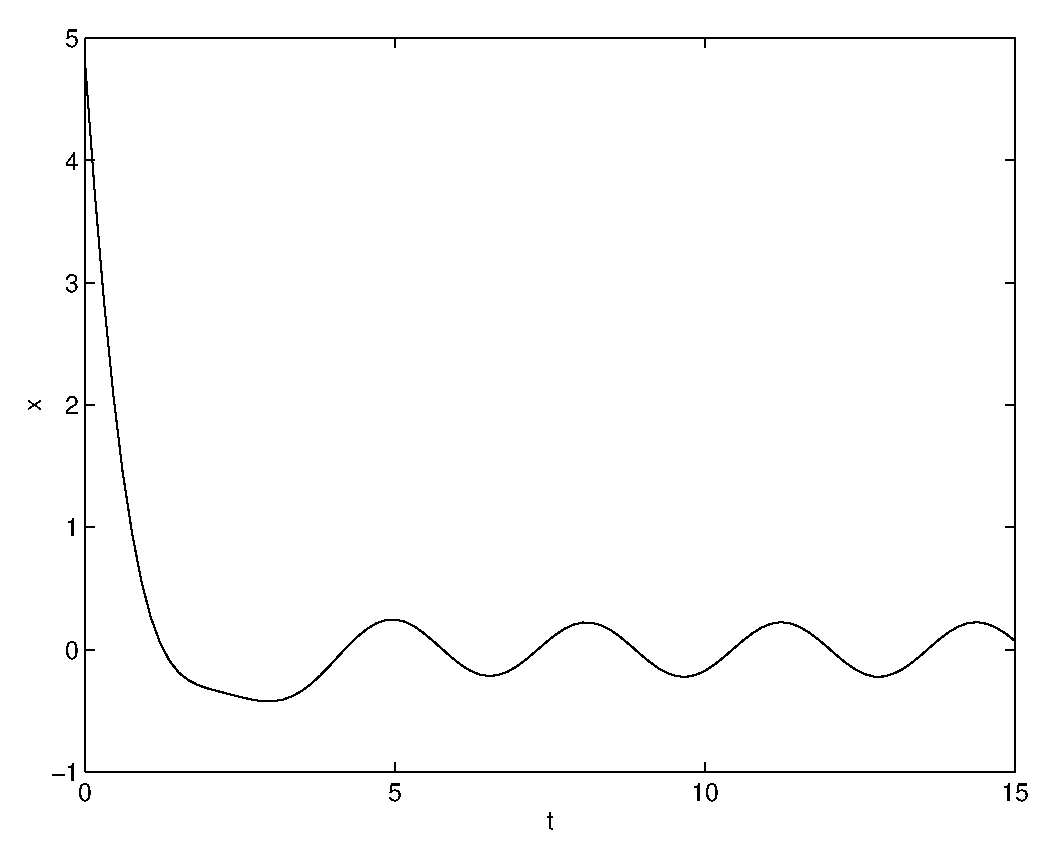
\psfig{file=exfigure/12-5-2.eps,width=3.0in}}
                \exercap{c12.5.2}
\end{figure}


\exer{c12.5.3}
Compute
\[
\lim_{\omega \rightarrow 1} x_\omega(t) =
\lim_{\omega \rightarrow 1}\left(\cos t + \frac{1}{1 - \omega^2}
(\cos(\omega t) - \cos t)\right) =
\cos t + \lim_{\omega \rightarrow 1}\frac{\cos(\omega t) - \cos t}
{(1 - \omega)(1 + \omega)}.
\]
Since $\dps \lim_{\omega \rightarrow 1}(1 + \omega) = 2$, we can write
\[
\lim_{\omega \rightarrow 1} x_\omega(t) =
\cos t - \frac{1}{2}\lim_{\omega \rightarrow 1}
\frac{\cos(\omega t) - \cos t}{\omega - 1}.
\]
Now, let $f(\omega) = \cos(\omega t)$.  Then
\[
\begin{array}{rcl}
\dps \lim_{\omega \rightarrow 1} x_\omega(t) & = &
\cos t - \dps \frac{1}{2}\lim_{\omega \rightarrow 1}
\frac{f(\omega) - f(1)}{\omega - 1} \\
& = & \cos t - f'(1) \\
& = & \cos t + \frac{1}{2}\left.t\sin(\omega t)\right|_{\omega = 1} \\
& = & \cos t + \frac{1}{2}t\sin t \\
& = & x_1(t).
\end{array}
\]

\exer{c12.5.a}  \ans Resonance occurs.

\soln  The internal frequency and the forcing frequency both equal $2$.

\newpage
\exer{c12.5.b} \ans Beats occur.

\soln  The internal frequency equals $4$ and the forcing frequency equals
$3.9$.  These are approximately equal and beats occur.

\exer{c12.5.c} \ans Neither beats nor resonance occur.

The internal frequency equals $3$ and the forcing frequency equals
$1$. These are far enough apart so that beats do not occur.

\exer{c12.5.d} \ans Resonance occurs.

\soln  The internal frequency and the forcing frequency both equal $3$.


\exer{c12.5.4}
The characteristic polynomial is $p(\lambda)=(\lambda^2+1)(\lambda^2+\omega^2)$. 
The roots of $p$ are $\pm i$ and $\pm\omega i$.  Therefore, solutions to the
inhomogeneous second order equations are linear combinations of sines and cosines with
two frequencies, that is, solutions are two-frequency motions.  Resonance occurs
when the eigenvalues are multiple, that is, when $\omega=\pm 1$.  Solutions to the
fourth order equation whose characteristic polynomial is $p$ are then linear
combinations of $\cos t$, $\sin t$, $t\cos t$, and $t\sin t$.  These factors of $t$ 
lead to resonant unbounded growth.
\end{document}
